\documentclass[../Head/Main.tex]{subfiles}
\begin{document}
\subsubsection{Sensor based planner}
\label{subsubsec:tangentBug}
The tangent bug algorithm have been implemented in a class called \texttt{motion\_planning} containing the methods.
\begin{itemize}
	\item \texttt{tanget\_bug\_algorithm(ct::current\_position pos, std::vector<ct::room> Rooms)}
	\item \texttt{homogeneous\_transformation(ct::current\_position robot, cv::Point goal})
\end{itemize}
This methods uses fuzzy logic to controlled the robot as explained in section \ref{subsec:searhStrategyDesign}. The \texttt{tanget\_bug\_algorithm(p,R)} takes the current position of the robot and a vector of room locations as inputs. Also this method gets the information about the shortest distance to obstacles from the robots LIDAR sensor which must be known for the robot to navigate along obstacles and avoid hitting them. The method \texttt{homogeneous\_transformation(r,g}) takes the current position of the robot and a goal location as inputs. This method is critical for the implementation of the tangent bug algorithm because it returns an orientation relative to the robot to the goal location. This method is actually used twice in the \texttt{tanget\_bug\_algorithm(p,R)} because both the orientation to the goal location as well as the orientation towards the closest obstacle must be known to be fetch by the fuzzy controller so that the robot can be giving the proper motion to reach the target position. 

\begin{figure}[H]
  \begin{subfigure}[b]{0.59\textwidth}
    \centering
    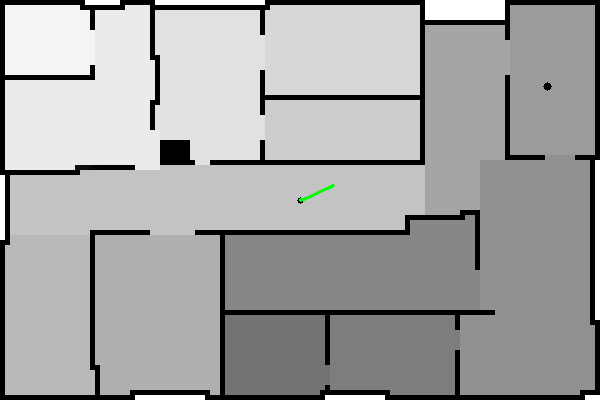
\includegraphics[width=0.9\textwidth]{tangentbug/Analysis1}
    \caption{The robots path from a initial position to a goal}
    \label{fig:tangentBugRobotPath1}
  \end{subfigure}
  \hfill
   \begin{subfigure}[b]{0.39\textwidth}
    \centering
    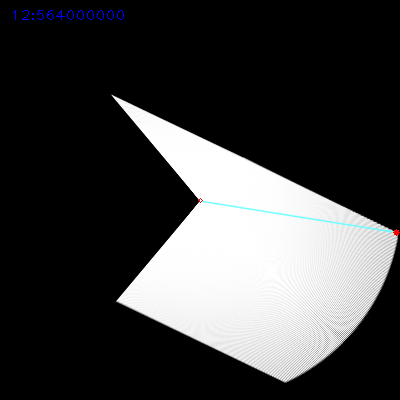
\includegraphics[width=0.9\textwidth]{tangentbug/Analysis2}
    \caption{Closest boundary on an obstacle to goal}
    \label{fig:closestBoundaryOnObstacle1}
  \end{subfigure}
  \end{figure}
  
\begin{figure}[H]
  \begin{subfigure}[b]{0.59\textwidth}
    \centering
    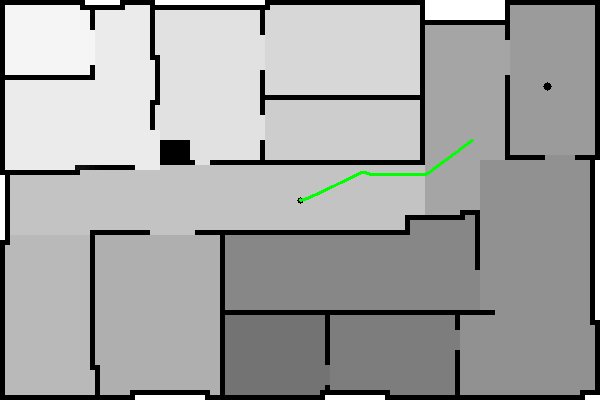
\includegraphics[width=0.9\textwidth]{tangentbug/Analysis3}
    \caption{The robots path from a initial position to a goal}
    \label{fig:tangentBugRobotPath2}
  \end{subfigure}
  \hfill
   \begin{subfigure}[b]{0.39\textwidth}
    \centering
    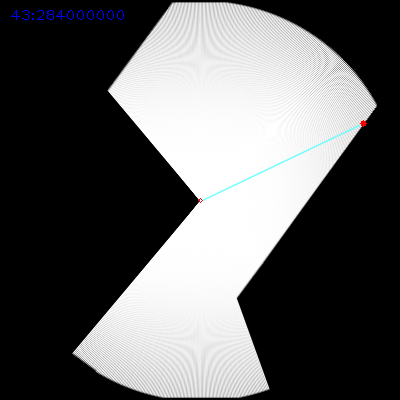
\includegraphics[width=0.9\textwidth]{tangentbug/Analysis4}
    \caption{Closest boundary on an obstacle to goal}
    \label{fig:closestBoundaryOnObstacle2}
  \end{subfigure}
  \end{figure}
  
  \begin{figure}[H]
  \begin{subfigure}[b]{0.59\textwidth}
    \centering
    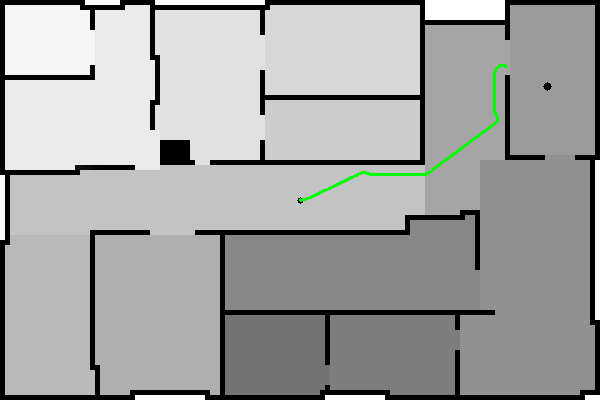
\includegraphics[width=0.9\textwidth]{tangentbug/Analysis5}
    \caption{The robots path from a initial position to a goal}
    \label{fig:tangentBugRobotPath3}
  \end{subfigure}
  \hfill
   \begin{subfigure}[b]{0.39\textwidth}
    \centering
    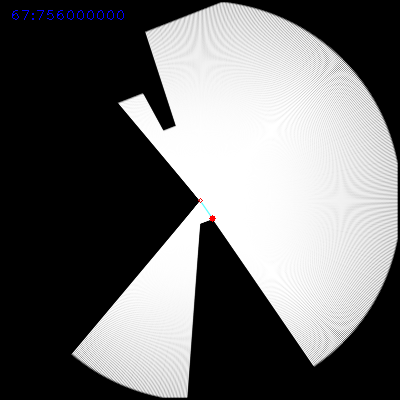
\includegraphics[width=0.9\textwidth]{tangentbug/Analysis6}
    \caption{Closest boundary on an obstacle to goal}
    \label{fig:closestBoundaryOnObstacle3}
  \end{subfigure}
\end{figure}
  
As mentioned in the design phase of constructing the tangent bug algorithm the robot follows the obstacle which minimizes the distance from the robots position to the boundary on the obstacle and from that point on the boundary to the goal. Figure (\ref{fig:tangentBugRobotPath1}) shows the path of the robot from an initial position to the target. Figure (\ref{fig:closestBoundaryOnObstacle1}) illustrates that point on the obstacle that minimises the complete path to the target if the robot is in an obstacle following behaviour. The boundary following behaviour only happens if an obstacle is blocking the way towards the goal. A number of test were conducted on the tangent bug algorithm and thereby the fuzzy control to test the implementation. The test can be seen in appendix (\ref{subsec:testMotionPlanning}).   

\begin{figure}[H]
	\begin{subfigure}[b]{0.49\textwidth}
    	\centering
    	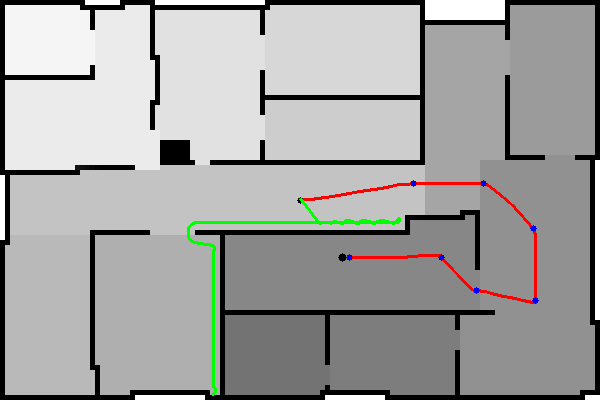
\includegraphics[width=0.9\textwidth]{Modelbased_vs_Sensorbased/brushfireAndBugTest12}
    	\caption{The robots travelling path from the origin to the target}
    	\label{fig:tangentBugAnalyseTest1}
  	\end{subfigure}
    \hfill
   	\begin{subfigure}[b]{0.49\textwidth}
    	\centering
    	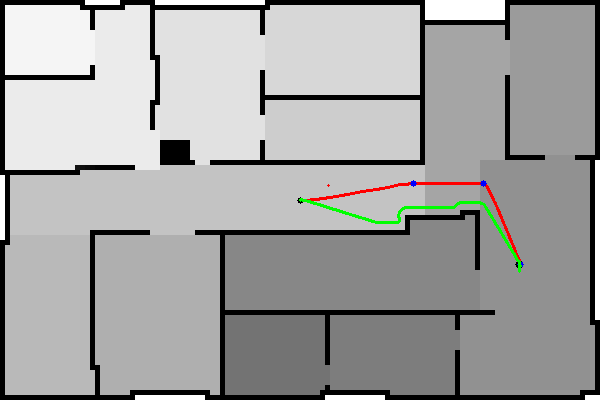
\includegraphics[width=0.9\textwidth]{Modelbased_vs_Sensorbased/brushfireAndBugTest11}
    	\caption{The robots travelling path from the origin to the target}
    	\label{fig:tangentBugAnalyseTest2}
  	\end{subfigure}
\end{figure}
  
The test showed that through a number of runs the average distance from the closest obstacles was 1.6 meters with a success rate of finding rooms at 64.3 \%. From figure (\ref{fig:tangentBugAnalyseTest1}) a scenario in which the tangent bug fails to reach a target location can be seen. The bug algorithm simply gets stuck in a corner, where the fuzzy controller also seems to have some limitations. The green line indicates the path of the sensor based planner and the red line the model based planner. On the other hand in figure (\ref{fig:tangentBugAnalyseTest2}) it performs quite well and follows the obstacles as intended. It is also worth noting that when the tangent bug finds its target location, it outperforms the model based planner regarding distance travelled. The closes distance to an obstacle was found to be 0.4 meters which satisfies the specification requirements. 
\end{document}